\documentclass[11pt]{article}
\usepackage{fontspec}
\usepackage[utf8]{inputenc}
\setmainfont{Bodoni 72 Book}
\usepackage[paperwidth=9in,paperheight=12in,margin=1in,headheight=0.0in,footskip=0.5in,includehead,includefoot,portrait]{geometry}
\usepackage[absolute]{textpos}
\TPGrid[0.5in, 0.25in]{23}{24}
\parindent=0pt
\parskip=12pt
\usepackage{nopageno}
\usepackage{graphicx}
\graphicspath{ {./images/} }
\usepackage{amsmath}
\usepackage{tikz}
\newcommand*\circled[1]{\tikz[baseline=(char.base)]{
            \node[shape=circle,draw,inner sep=1pt] (char) {#1};}}

\begin{document}

\begin{center}
\huge FOREWORD
\end{center}

\begingroup
\begin{center}
\leftskip0.5in
``Appellations que vous trouverez ci-après, dans ce Livre: de même que la véritable composition de \textit{la Verge Foudroyante}, et ses effets qui font trembles les Esprits, et dont Dieu se servit pour armer son Ange, qui chassa Adam et Eve du paradis terrestre, et de laquelle Dieu frappa les Anges rebelles, précipitant leur orgueils dans des Abymes les plus épouvantables, par la force de cette Verge qui forme des nuées, qui disperse les ouragans et les fait tomber sur quelle partie de la Terre que vous voulez."
\rightskip\leftskip
\phantom{text} \hfill - J. Karter
\end{center}
\endgroup


\begingroup
\begin{center}
\rule{\textwidth}{1.6pt}\vspace*{-\baselineskip}\vspace*{1pt}
\rule{\textwidth}{0.4pt}\\[\baselineskip]
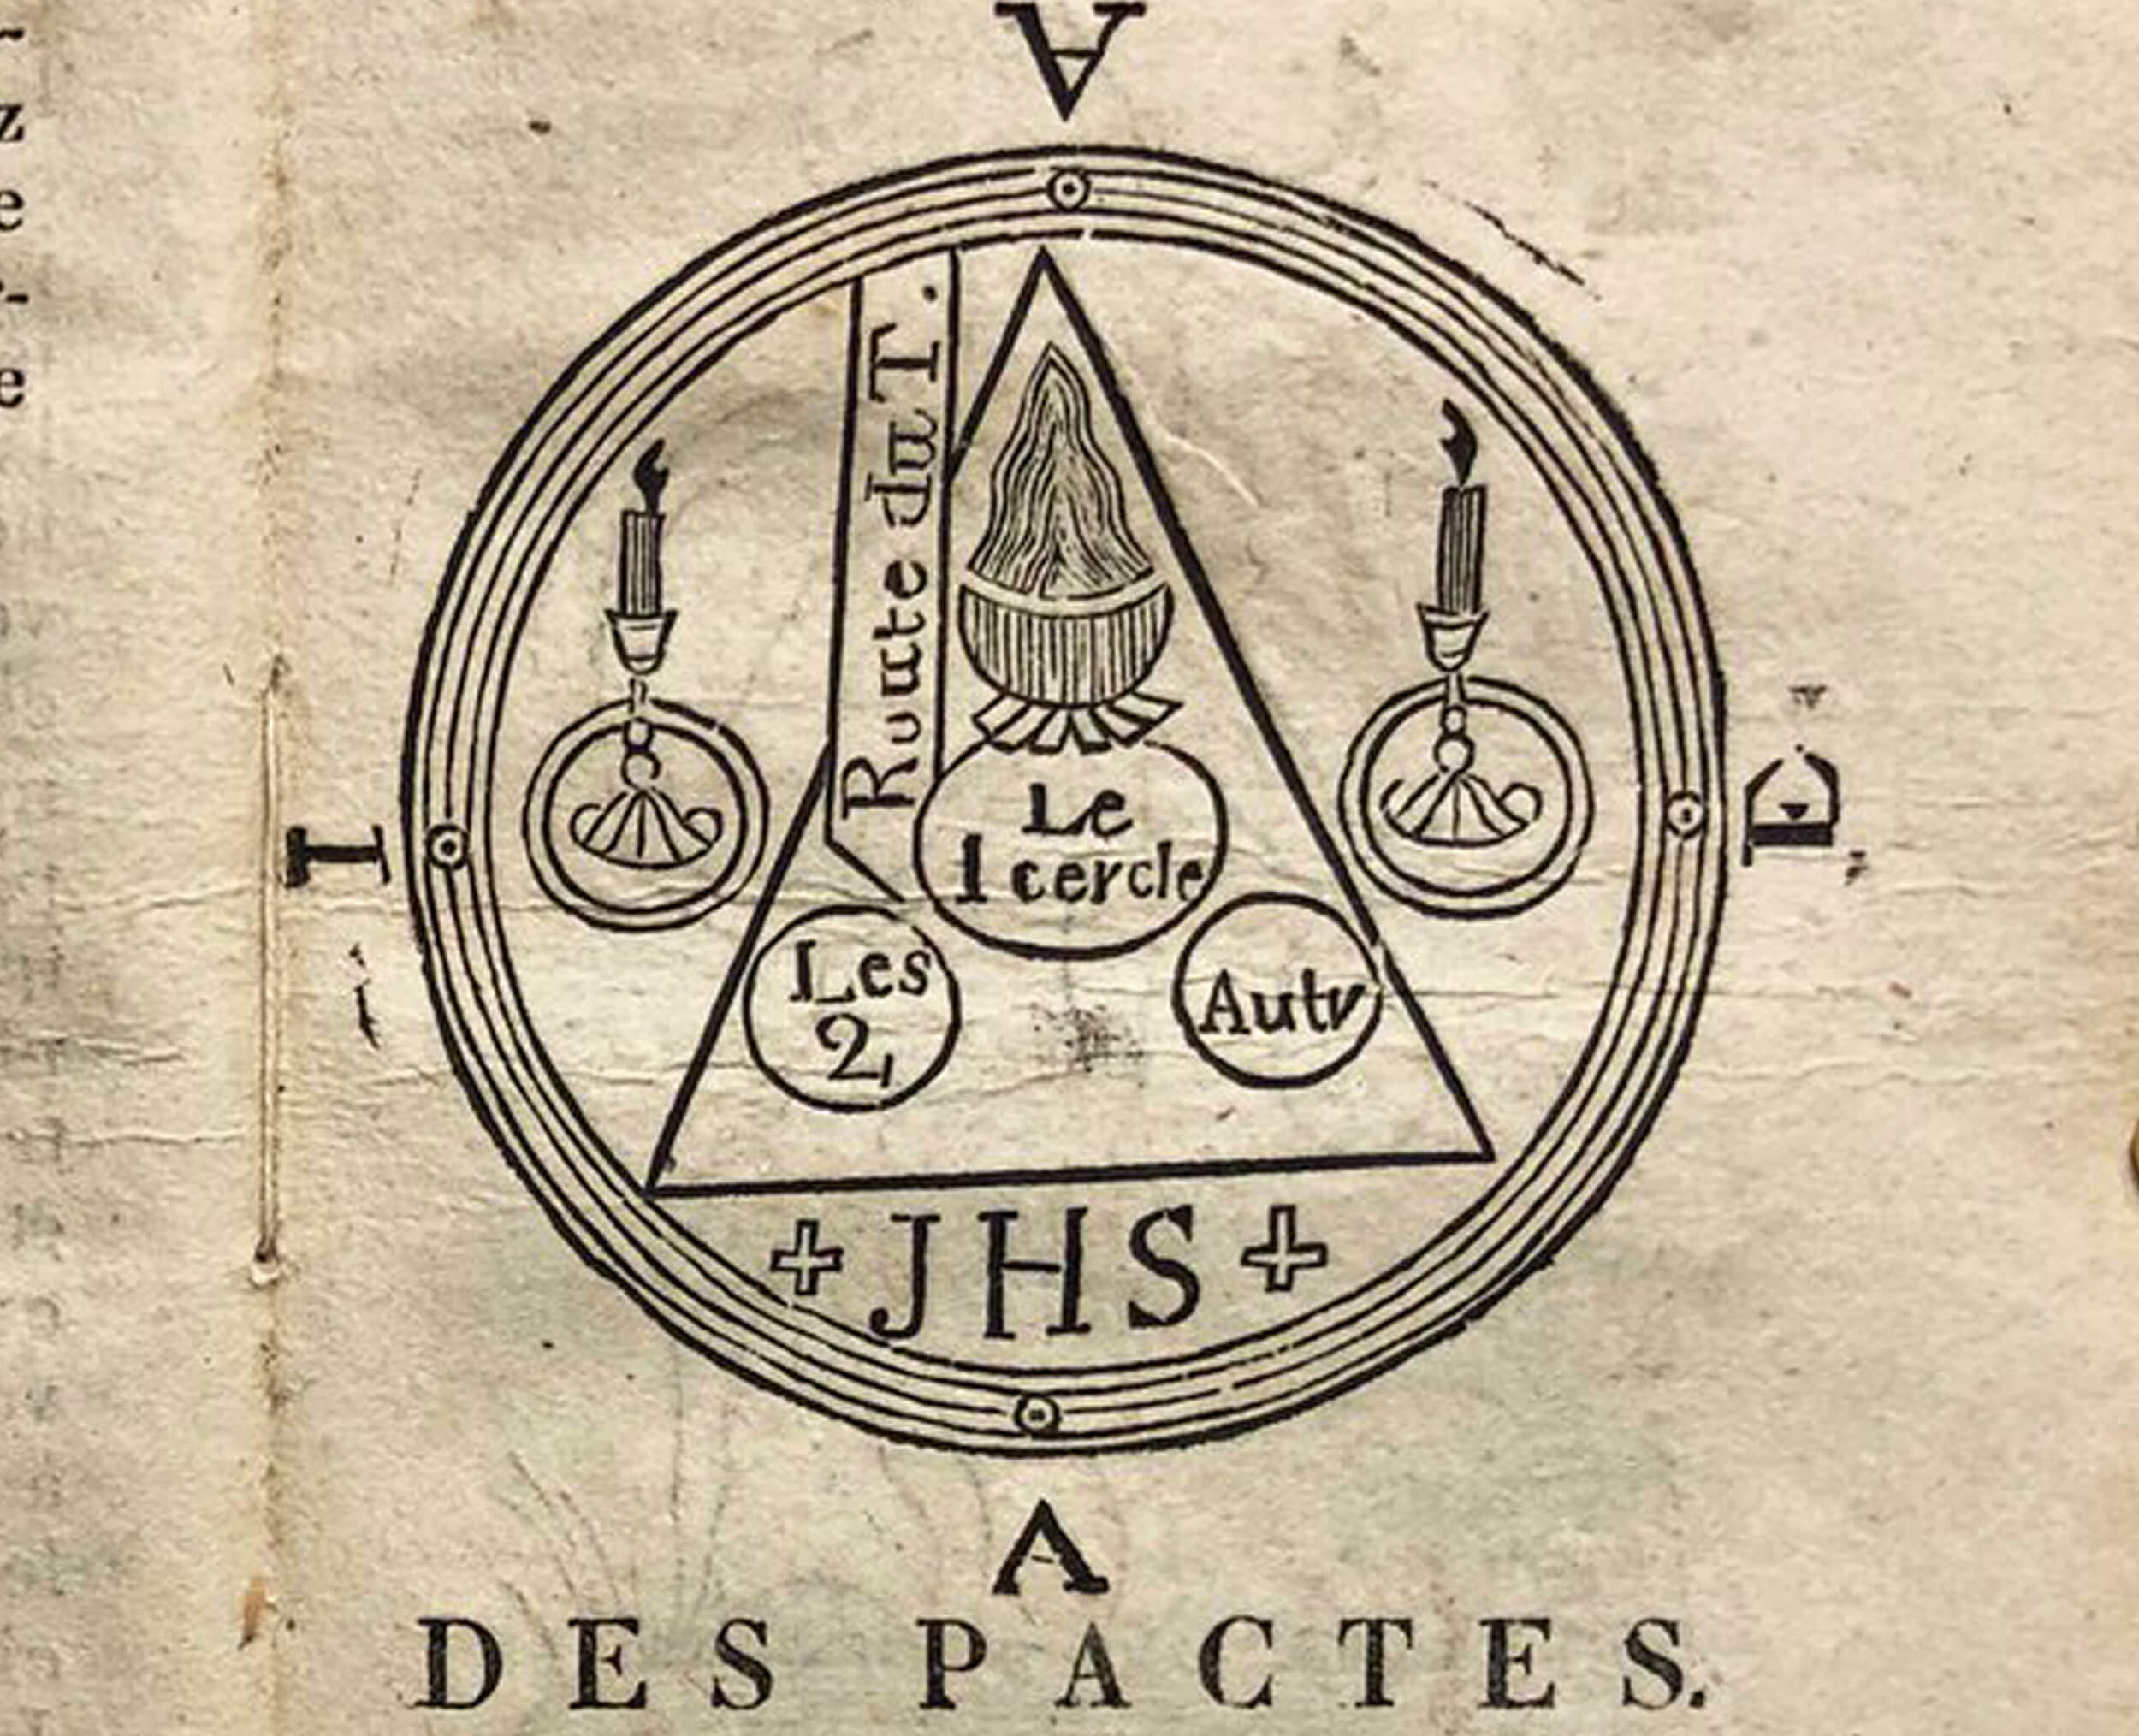
\includegraphics[scale=0.20]{verge.jpeg}
\rule{\textwidth}{0.4pt}\vspace*{-\baselineskip}\vspace{2pt}
\rule{\textwidth}{1.6pt}\\[\baselineskip]
\end{center}
\endgroup

\begingroup
\begin{center}
\leftskip0.5in
``Appellations that you will find below, in this Book: as well as the true composition of \textit{the Lightning Rod}, and its effects which make the Spirits tremble, and which God used to arm his Angel, who expelled Adam and Eve of the earthly paradise, and from which God struck the rebellious Angels, precipitating their pride into the most dreadful Abysses, by the force of this Rod which forms clouds, which disperses hurricanes and causes them to fall on what part of the Earth you wish."
\rightskip\leftskip
\phantom{text} \hfill - J. Karter ( English approximation )
\end{center}
\endgroup


\end{document}
